\documentclass[]{article}
\usepackage[T1]{fontenc}
\usepackage{lmodern}
\usepackage{amssymb,amsmath}
\usepackage{ifxetex,ifluatex}
\usepackage{ctan}
\usepackage{tikz}
\usepackage{graphicx}
\usepackage{fixltx2e} % provides \textsubscript
% use upquote if available, for straight quotes in verbatim environments
\IfFileExists{upquote.sty}{\usepackage{upquote}}{}
\ifnum0\ifxetex1\fi\ifluatex1\fi=0 % if pdftex
  \usepackage[utf8]{inputenc}
\else % if luatex or xelatex
  \ifxetex\usepackage{mathspec}
    \usepackage{xltxtra,xunicode}
  \else
    \usepackage{fontspec}
  \fi
  \defaultfontfeatures{Mapping=tex-text,Scale=MatchLowercase}
  \newcommand{\euro}{€}
\fi
% use microtype if available
\IfFileExists{microtype.sty}{\usepackage{microtype}}{}
\ifxetex\usepackage[setpagesize=false, % page size defined by xetex
              unicode=false, % unicode breaks when used with xetex
              xetex]{hyperref}
\else
  \usepackage[unicode=true]{hyperref}
\fi
\hypersetup{breaklinks=true,
            bookmarks=true,
            pdfauthor={},
            pdftitle={},
            colorlinks=true,
            citecolor=blue,
            urlcolor=blue,
            linkcolor=magenta,
            pdfborder={0 0 0}}
\urlstyle{same}  % don't use monospace font for urls
\setlength{\parindent}{0pt}
\setlength{\parskip}{6pt plus 2pt minus 1pt}
\setlength{\emergencystretch}{3em}  % prevent overfull lines
\setcounter{secnumdepth}{0}

\author{}
\date{}

\begin{document}
\section{Examples}\label{examples}

\subsection{Synthesis of Collision Avoidance
Protocol}\label{synthesis-collision-avoidance-protocol}

\subsubsection{Problem statement}\label{problem-statement}

In this scenario we have $n$ UAVs, $m$ altitude layers and $q$ locations of
interest. A UAV can ascend or descend to the altitude layer above or
below its current altitude layer. A location is a predefined
point on an altitude layer. Our aim is to automatically synthesize a
control protocol that guarantees the following:

\begin{enumerate}
\def\labelenumi{\arabic{enumi}.}
\itemsep1pt\parskip0pt\parsep0pt
\item
  Each UAV is able to visit, infinitely often, all of the locations of
  interest.
\item
  No Collision between UAVs.
\end{enumerate}

\subsubsection{Approach}\label{approach}
\begin{figure}[htp]
\begin{tikzpicture}
    \node[anchor=south west,inner sep=0] (image) at (0,0,0) {\frame{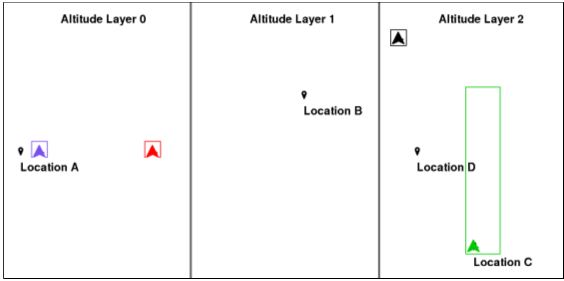
\includegraphics[width=4in]{figs/ca_1.png}}};
    \begin{scope}[x={(image.south east)},y={(image.north west)}]
        %% next four lines will help you to locate the point needed by forming a grid. comment these four lines in the final picture.↓
  %      \draw[help lines,xstep=.1,ystep=.1] (0,0) grid (1,1);
%        \draw[help lines,xstep=.05,ystep=.05] (0,0) grid (1,1);
%        \foreach \x in {0,1,...,9} { \node [anchor=north] at (\x/10,0) {0.\x}; }
%        \foreach \y in {0,1,...,9} { \node [anchor=east] at (0,\y/10) {0.\y};}
        %% upto here↑
        \draw[dashed,-latex] (0.925,0.8) -- +(-0.7in,0.7in)node[align=left] {the operating region for the purple UAV};
        \draw[dashed,-latex] (0.82,0.45) -- +(-.8in,-0.6)node[align=left] {UAV};
        \draw[dashed,-latex] (0.925,0.15) -- +(-.3in,-0.25)node[align=left] {a pre-defined location};
    \end{scope}
\end{tikzpicture}
    \label{fig:ca}
    \caption{}
\end{figure}

Our approach to this problem is centered around the idea of UAVs'
operating regions. An operating region for a UAV is a polygon on the
UAV's current altitude layer. We assume That the UAV will only fly
within its operating region. With this assumption, we can guarantee that
no collision will happen if the UAV with intersected operating region
remain still until the intersection is resolved.


At each turn, each UAV will signal an intention to visit a specific location or to remain still. We assume that there cannot be two UAVs intending to go to the same location to prevent deadlocks. We use this intention signal to update the operating regions for all the UAVs so that the intended locations are inside the operating regions of the UAVs. The algorithm for updating the operating regions ensures that the updated regions for all the UAVs do not intersect. Currently, there is no guarantee that the algorithm will terminate. The algorithm includes reshaping the operating regions and moving the UAVs to nearby location to resolve operating regions intersections. The UAV will then be given the command to go to location it intended to go to. It is assumed that the UAV will reach the location in one time step. 

\subsubsection{Problem setup}\label{problem-setup}

We model this problem by assigning three output variables $l_{i} \in L$ where $L$ is the set of indices of the altitude layers, $p_{i},t_{i} \in P$ where $P$ is the set of indices of locations, and $(n-1)$ input variables $c_{ij}  \in B$ where B is the boolean set and $c_{ij} = c_{ji}$ to each UAV$_{i}$ where $i,j \in U$, the set of indices for the UAVs. The variables are defined as follows: 

\begin{itemize}
\item
  \textbf{$l_{i}$:} the altitude layer for UAV$_{i}$ to ascend or descend to.
\item
  \textbf{$p_{i}$:} the location for UAV$_{i}$ to head to.
\item
  \textbf{$t_{i}$:} the intention of  UAV$_{i}$.
\item
  \textbf{$c_{ij}$:} true if the operating region for
  UAV$_{i}$ intersects with that of UAV$_{j}$ and false otherwise.
\end{itemize}

At each time instance, the synthesized controller takes the variables $c_{ij}$ as inputs and outputs $l_{i}$, $g_{i}$, $t_{i}$ for each UAV\@.

\subsubsection{System specifications}\label{system-specifications}

\begin{itemize}
\itemsep1pt\parskip0pt\parsep0pt
\item
  UAV$_{i}$ can only go to the locations that are in the same altitude
  layer: $(\bigwedge\limits_{i \in U} \square (l_{i} = x \implies p_{i} = x \bigvee\limits_{i \in P} p_{i} = stay))$
\item
  UAV$_{i}$ and UAV$_{j}$ must not be at the same altitude layer if
  $c_{ij}$ is true (their operating regions intersect): $(\bigwedge\limits_{i\in U} \bigwedge\limits_{j\in U} \square (c_{ij} \implies l_{i} \neq l_{j}))$
\item
  If UAV$_{i}$ is given a command to go to $x$ then it must have
  signaled its intent at the previous step:$(\bigwedge\limits_{i \in U} \square (p_{i} = x \implies t_{i} = x))$
\item
  UAV$_{i}$ will eventually be sent the command to go to $x$: $(\bigwedge\limits_{i \in U} \square \lozenge (p_{i} = x))$
\end{itemize}

\subsubsection{Environment assumptions}\label{environment-assumptions}


We assume that if two UAVs have intersecting operating regions and one
of the UAVs signaled an intention to go to a location then the
intersection will be resolved: ($\square  \lozenge \bigwedge\limits_{i \in U}\bigwedge\limits_{j \in U} ( \lnot c_{ij})$).


\subsection{Synthesis of VIP Escort Protocol}\label{vip-escort}

\subsubsection{Problem statement}\label{problem-statement}

In this scenario we have one main UAV we call ``VIP'', multiple
``escort'' UAVs, and multiple pre-defined locations on the map. These locations are shown in green in fig \ref{fig:vip}. Our aim is
to automatically synthesize a control protocol that guarantees the
following:
\begin{figure}[htp]
    \centering
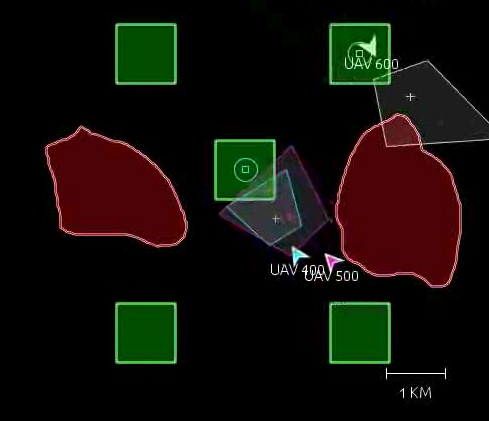
\includegraphics[scale=.4]{figs/vip.png}
    \caption{}
    \label{fig:vip}
\end{figure}

\begin{enumerate}
\def\labelenumi{\arabic{enumi}.}
\itemsep1pt\parskip0pt\parsep0pt
\item
  The VIP must not move from one location to another without being
  followed by one of the escorts.
\item
  The VIP cannot visit certain locations until at least one of the
  escorts have inspected the location within the last $x$ steps. A location is considered inspected if an escort flies over the location.
\item
    In order for the UAVs not to pass through the prohibited regions shown in red in fig \ref{fig:vip}, the UAVs must follow certain paths between the locations in green. For example, to go from the bottom right location to the upper right, the UAVs must pass through the middle location so that they do not fly over the prohibited regions.
\end{enumerate}

\subsubsection{Problem setup}\label{problem-setup}

We model this problem by assigning two output variables $g_{i} \in P$ where $P$ is the set of location indices and $t_{i}\in B$ where $B$ is the boolean set and one input variable $s_{i} \in P$ to each escort UAV$_{i}$ where $i \in U$, the set of escort UAV indices. As for the VIP we assign one input variable $p \in P$ and one output variable $q \in P$. In addition, we assign a variable $r_{i} \in B$ where $i \in P$. The variables are defined as follows:

\begin{itemize}
        \item
            $g_{i}$: the location for UAV$_{i}$ to go to.
        \item
            $t_{i}$: if true UAV$_{i}$ will start following the VIP\@.
        \item
            $s_{i}$: the current location of UAV$_{i}$.
        \item
            $p$: the current location of the VIP.
        \item
            $q$: the location for the VIP to go to.
        \item
            $r_{i}$: true if location$_{i}$ was inspected in the past.
\end{itemize}


\subsubsection{System specifications}\label{system-specifications}
The system specifications for synthesizing the controller consist of four sets of LTL specifications.1) The escort must be at the same location as the VIP to be able to follow it $\square (t_{i} \implies p = s_{i})$.2) The VIP cannot fly from a location to another without being followed by another UAV $\square(\bigwedge\limits_{i\in U}\lnot ti_{i} \implies \Circle p = p$).3) The VIP must always eventually visits a set of locations: $\bigwedge\limits_{p\in P}\square \lozenge q$.4) a set of locations must eventually be inspected $\bigwedge\limits_{i\in P}\square \lozenge r_{i}$.
\subsubsection{Environment assumptions}\label{environment-assumptions}
We make three sets assumptions on the environment. First, the location is considered inspected when an escort visits the location, $\square (s_{i} \implies r_{i})$. Second, an inspected location remains inspected. It is also possible to set an expiration timer for the location to switch back not inspected: $\square (r_{i} \implies \Circle r_{i})$. The last assumption is that all UAVs will reach their destinations they were commanded to fly to by the next time step: $\square (g_{i} \implies \Circle s_{i})$.

\end{document}
